\documentclass[sigconf]{acmart}

\AtBeginDocument{%
  \providecommand\BibTeX{{Bib\TeX}}}

\setcopyright{none}
\settopmatter{printacmref=false}
\renewcommand\footnotetextcopyrightpermission[1]{}

\graphicspath{{figures/}}
\usepackage{booktabs}
\usepackage{dblfloatfix}
\usepackage{placeins}
\usepackage{flafter}
\usepackage{balance}
\usepackage{subcaption}
\setlength{\floatsep}{4pt plus 1pt minus 1pt}
\setlength{\textfloatsep}{6pt plus 1pt minus 2pt}
\setlength{\intextsep}{4pt plus 1pt minus 1pt}
\setlength{\dblfloatsep}{4pt plus 1pt minus 1pt}
\setlength{\dbltextfloatsep}{6pt plus 1pt minus 2pt}
\setlength{\abovecaptionskip}{4pt}
\setlength{\belowcaptionskip}{2pt}
\renewcommand{\topfraction}{0.9}
\renewcommand{\bottomfraction}{0.9}
\renewcommand{\dbltopfraction}{0.9}
\renewcommand{\textfraction}{0.07}
\renewcommand{\floatpagefraction}{0.8}
\renewcommand{\dblfloatpagefraction}{0.8}

\begin{document}

\title[Discrete Embedding Grids with ACOM]{Discrete Embedding Grids with ACOM}

\author{Haseeb Raza}
\affiliation{%
  \institution{ELTE}
  \city{Budapest}
  \country{Hungary}}
\email{haseeb.javed715@gmail.com}

\renewcommand{\shortauthors}{Haseeb Raza}

\begin{abstract}
We evaluate whether document embeddings can be placed on a discrete two-dimensional semantic grid with an ACOM-style swap optimizer. On a balanced five-class 20 Newsgroups benchmark, the strongest archived ACOM variant improves neighborhood preservation from 0.134 to 0.367 and trustworthiness from 0.567 to 0.787 relative to the baseline ACOM configuration. Tuned ACOM exceeds PCA on those two local-structure metrics, but t-SNE and UMAP remain stronger overall on the benchmark. A scaling study shows that the method remains operational through 200 documents while quality peaks around 100 documents and then declines. These results support ACOM as an interpretable discrete mapper rather than a raw metric leader over strong continuous baselines.

\end{abstract}

% Conference metadata kept minimal for this draft.
\acmConference[Intelligent Robotics FAIR 2026]{Intelligent Robotics FAIR 2026}{}{}

% TODO: Replace with real ACM CCS concepts if required by the venue.
% \begin{CCSXML}
% \end{CCSXML}
% \ccsdesc[500]{TODO}

\keywords{document embeddings, discrete semantic mapping, ACOM, dimensionality reduction, semantic grids}

\maketitle

\section{Introduction}

Most document embedding visualizations are continuous 2D projections. This paper focuses on a different problem: placing documents on an explicit semantic grid. We study that setting with an ACOM-style swap optimizer and compare the resulting discrete map against PCA, t-SNE, and UMAP.

The supported claim is narrow. Tuned ACOM improves strongly over the baseline and beats PCA on neighborhood preservation and trustworthiness, but it does not outperform t-SNE or UMAP overall. We present ACOM as a discrete and interpretable mapping method rather than a universal replacement for continuous projections.

% TODO: Add related-work citations once the bibliography is prepared.

\section{Method and Experimental Setup}

\subsection{Dataset}

The dataset is the 20 Newsgroups dataset~\cite{lang1995newsweeder}, a standard benchmark for text categorization containing approximately 18,000 posts across 20 newsgroup categories. We obtained the dataset via scikit-learn's \texttt{fetch\_20newsgroups} loader~\cite{pedregosa2011sklearn}, which downloads the \texttt{20news-bydate} archive from the original distribution. The five categories used are \mbox{\texttt{comp.graphics}}, \mbox{\texttt{rec.sport.baseball}}, \mbox{\texttt{sci.med}}, \mbox{\texttt{sci.space}}, and \mbox{\texttt{talk.politics.misc}}. We sampled 10 documents per category per split, giving 50 train and 50 test documents for 100 documents total. Preprocessing removed headers, footers, and quoted reply text. Embeddings use the all-MiniLM-L6-v2 model from the sentence-transformers library~\cite{reimers2019sentencebert}, producing 384-dimensional embeddings.

\subsection{Methods Compared}

Principal Component Analysis (PCA) \cite{pearson1901pca} is a linear projection that preserves directions of maximum variance in the data. t-distributed Stochastic Neighbor Embedding (t-SNE) \cite{vandermaaten2008tsne} is a nonlinear method that preserves local neighborhood structure by minimizing the KL divergence between high- and low-dimensional pairwise similarity distributions. Uniform Manifold Approximation and Projection (UMAP) \cite{mcinnes2018umap} is a manifold learning method that balances local and global structure. The proposed ACOM mapper places each document on a discrete grid cell through iterative swap proposals evaluated against a cost function that attracts semantic neighbors and repels semantically distant grid neighbors. The strongest variant combines wider swap candidate search with annealed acceptance.

\subsection{ACOM Variants}

Seven ACOM configurations were evaluated in a controlled sweep, each isolating one design decision relative to the baseline. The variants are listed in Table~\ref{tab:variant-labels}. The baseline (I) uses greedy acceptance and a swap candidate breadth of 12. Variant II increases semantic neighbor coverage to k=10. Variant III extends the iteration budget. Variant IV expands the local neighborhood radius to 2. Variant V increases the repulsion weight. Variant VI widens the swap candidate search to 20. The tuned configuration (VII) combines variant VI with annealed acceptance, which permits occasional uphill moves to escape local minima.

\subsection{Metrics}

We evaluate all methods using the following metrics, computed against the same original embedding space.

\paragraph{Neighborhood Preservation}
Let $\mathcal{N}_k^H(i)$ and $\mathcal{N}_k^L(i)$ denote the $k$ nearest neighbors of point $i$ in the original embedding space and in the mapped space respectively. Neighborhood preservation is:
\begin{equation}
\text{NP} = \frac{1}{nk} \sum_{i=1}^{n} \left|\mathcal{N}_k^H(i) \cap \mathcal{N}_k^L(i)\right|
\end{equation}

\paragraph{Trustworthiness}
Trustworthiness~\cite{venna2006trustworthiness} measures whether points introduced as neighbors by the mapping are genuine neighbors in the original space:
\begin{equation}
T(k) = 1 - \frac{2}{nk(2n-3k-1)} \sum_{i=1}^{n} \sum_{j \in \mathcal{N}_k^L(i) \setminus \mathcal{N}_k^H(i)} (r(i,j) - k)
\end{equation}
where $r(i,j)$ is the rank of point $j$ in the original space sorted by distance from $i$.

\paragraph{Stress}
Stress measures disagreement between original pairwise distances and mapped pairwise distances:
\begin{equation}
\text{Stress} = \sqrt{\frac{\sum_{i<j}(d_{ij} - \hat{d}_{ij})^2}{\sum_{i<j} d_{ij}^2}}
\end{equation}
where $d_{ij}$ is the original cosine distance and $\hat{d}_{ij}$ is the Euclidean distance in the mapped space.

\paragraph{Silhouette Score}
The silhouette score~\cite{rousseeuw1987silhouette} measures cluster separation quality in the mapped space, ranging from $-1$ to $1$ where higher values indicate better-separated clusters.

% TODO: Add a concise algorithm box or pseudocode if the final venue page budget allows.

\section{Results}

\subsection{Qualitative Comparison}\label{sec:qualitative}

Figure~\ref{fig:qualitative-panel} summarizes the output types directly. ACOM produces an explicit grid assignment, while PCA, t-SNE, and UMAP remain continuous scatter layouts. This discrete-versus-continuous difference is the main qualitative motivation for the method.

\begin{figure*}[!t]
  \centering
  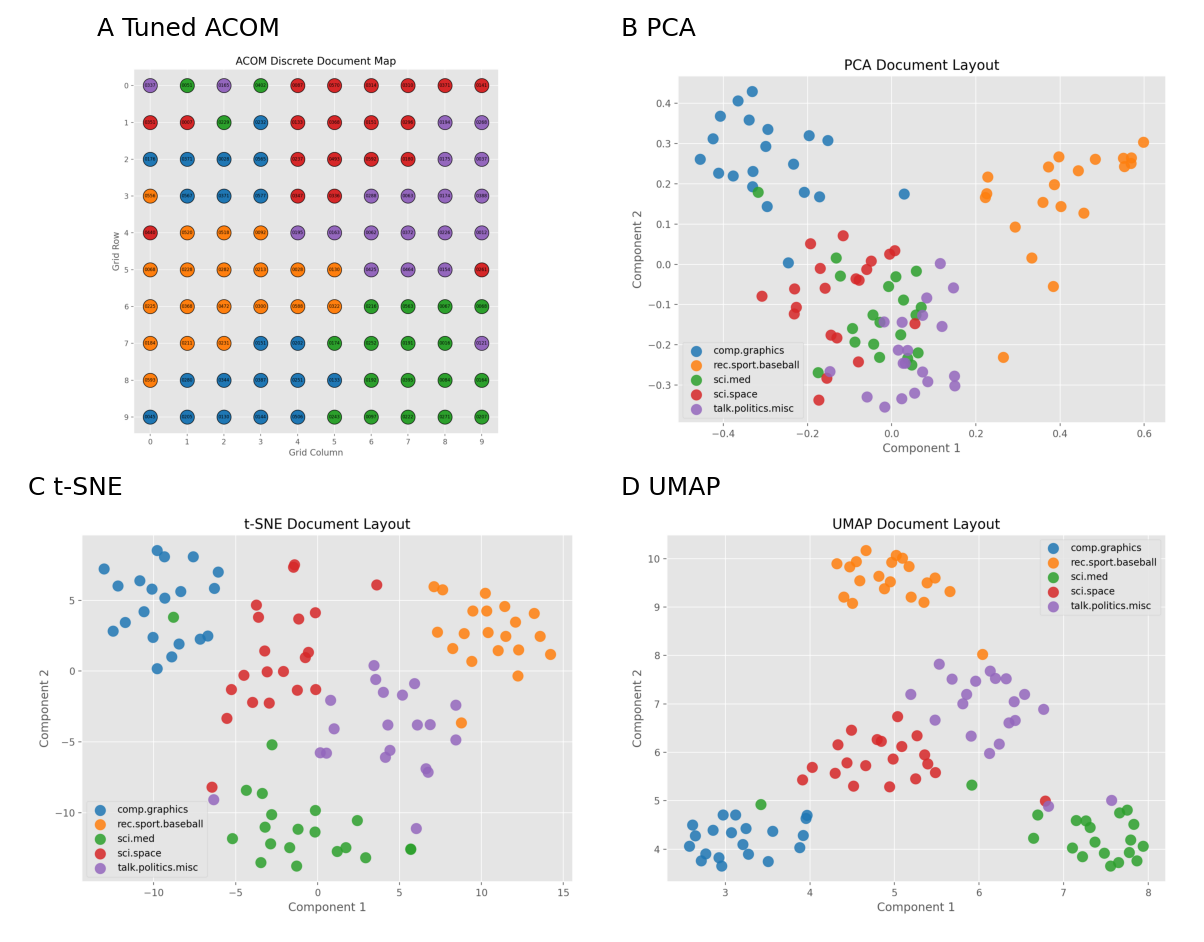
\includegraphics[width=0.78\textwidth]{qualitative_comparison_compact.png}
  \caption{Compact qualitative comparison on the 100-document benchmark: tuned ACOM grid (A), PCA (B), t-SNE (C), and UMAP (D). ACOM is the only method that yields an explicit discrete semantic grid rather than a continuous scatter layout.}
  \Description{A four-panel comparison figure showing the tuned ACOM grid and three baseline scatter plots on the same benchmark dataset.}
  \label{fig:qualitative-panel}
\end{figure*}

\subsection{Baseline vs. Tuned ACOM}\label{sec:baseline-vs-tuned}

The baseline ACOM configuration is weak on local-structure preservation: neighborhood preservation is 0.134 and trustworthiness is 0.567. The tuned variant raises those values to 0.367 and 0.787, respectively. Wider search gives the first substantial improvement, and annealed acceptance produces the final jump to the best saved result.

Figure~\ref{fig:baseline-vs-tuned} makes the same change visible in the map itself: the tuned layout forms more coherent local regions than the baseline grid. This baseline-to-tuned transition is one of the clearest positive results in the repository.

\begin{figure*}[!t]
  \centering
  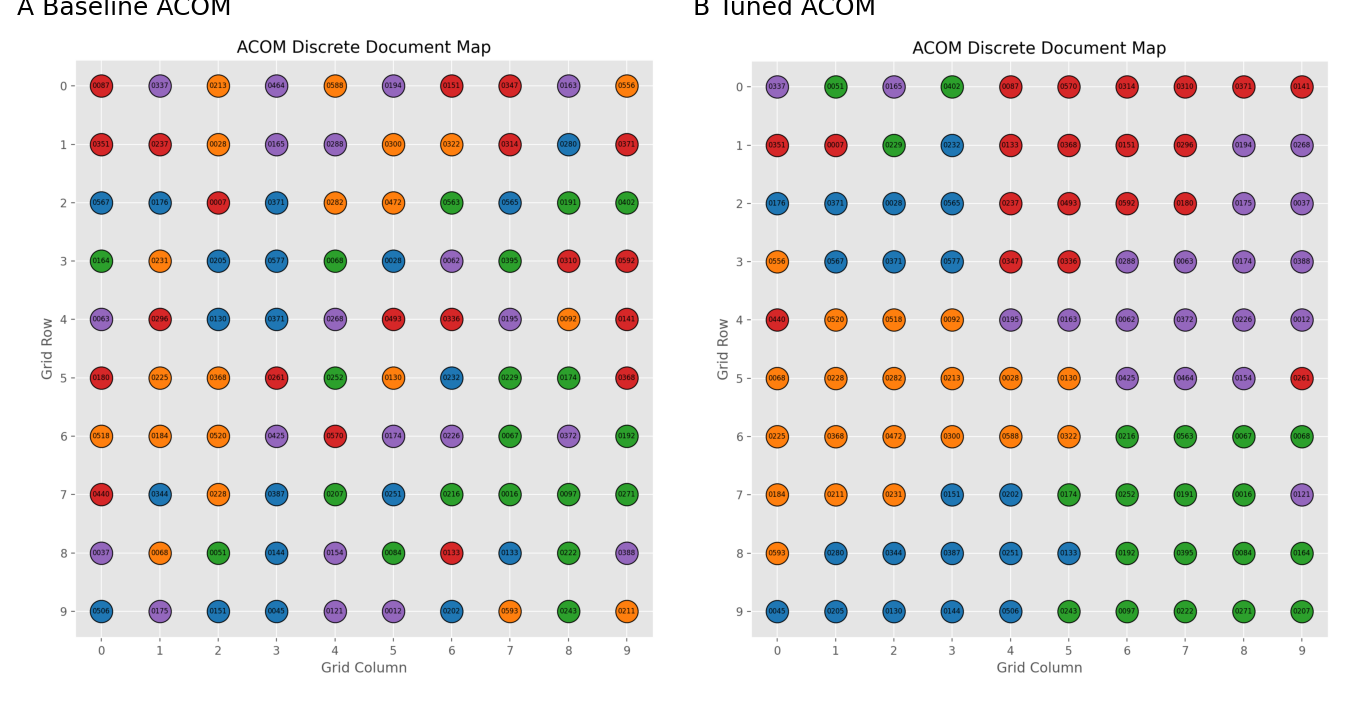
\includegraphics[width=0.78\textwidth]{baseline_vs_tuned_panel.png}
  \caption{Baseline versus tuned ACOM on the 100-document benchmark. The baseline grid (A) has neighborhood preservation 0.134 and trustworthiness 0.567, while the tuned grid (B) reaches 0.367 and 0.787. The improvement corresponds to wider swap search followed by annealed acceptance.}
  \Description{A two-panel figure comparing the baseline ACOM grid and the tuned ACOM grid on the same benchmark dataset.}
  \label{fig:baseline-vs-tuned}
\end{figure*}

\subsection{Variant Sweep and Model Selection}\label{sec:variant-sweep}

Figure~\ref{fig:variant-comparison} and Table~\ref{tab:acom-ablation} show that not all changes help equally. Increasing neighbors, iterations, or radius produces only modest gains, while stronger repulsion barely improves on the baseline. The first clear step comes from wider search (0.239 neighborhood preservation, 0.683 trustworthiness), and annealed acceptance then produces the tuned configuration.

\begin{figure*}[!t]
  \centering
  
\includegraphics[width=0.78\textwidth]{acom_variant_comparison.png}
  \caption{ACOM variant sweep. Wider search produces the first major gain over the baseline, and annealed acceptance yields the strongest final result. Variant labels I--VII are defined in Table~\ref{tab:variant-labels}.}
  \Description{A three-panel bar chart comparing ACOM variants on cost improvement, neighborhood preservation, and trustworthiness.}
  \label{fig:variant-comparison}
\end{figure*}

\begin{table}[!tb]
  \caption{Roman-numeral labels used for the ACOM variant sweep in Figure~\ref{fig:variant-comparison}.}
  \label{tab:variant-labels}
  \centering
  \small
  \begin{tabular}{ll}
    \toprule
    Label & Variant Description \\
    \midrule
    I & Baseline \\
    II & k=10 \\
    III & More Iterations \\
    IV & Radius 2 \\
    V & Strong Repulsion \\
    VI & Wider Search \\
    VII & Tuned (Wider Search + Annealed Acceptance) \\
    \bottomrule
  \end{tabular}
\end{table}

\begin{table}[!tb]
  \caption{ACOM variant sweep used for model selection. The baseline row is the untuned configuration; the tuned row combines wider swap search with annealed acceptance and gives the strongest result.}
  \label{tab:acom-ablation}
  \centering
  \scriptsize
  \begin{tabular}{lrrrlr}
    \toprule
    Variant & Search & Neigh. & Trust. & Accept. & Cost Impr. \\
    \midrule
    \textbf{Baseline} & 12 & \textbf{0.134} & \textbf{0.567} & greedy & 25.063 \\
    k=10 & 12 & 0.189 & 0.609 & greedy & 47.815 \\
    More Iter. & 12 & 0.191 & 0.637 & greedy & 48.711 \\
    Radius 2 & 12 & 0.188 & 0.625 & greedy & 56.417 \\
    Strong Repulse & 12 & 0.137 & 0.574 & greedy & 27.676 \\
    \textbf{Wider Search} & 20 & \textbf{0.239} & \textbf{0.683} & greedy & 66.307 \\
    \textbf{Tuned} & 20 & \textbf{0.367} & \textbf{0.787} & annealed & 87.815 \\
    \bottomrule
  \end{tabular}
\end{table}


\subsection{Final Benchmark Comparison}\label{sec:benchmark}

Table~\ref{tab:main-comparison} gives the final benchmark comparison against PCA, t-SNE, and UMAP. Tuned ACOM reaches neighborhood preservation 0.367 and trustworthiness 0.787, exceeding PCA on both metrics (0.329 and 0.758). However, PCA remains much better on stress (0.612 versus 5.107), and t-SNE and UMAP are stronger overall on the benchmark. The supported claim is therefore narrower: ACOM is competitive with PCA on the two local metrics while producing a discrete semantic grid that the continuous baselines do not provide.
The higher stress values arise because the discrete grid constraint limits the ability to preserve global distances compared with continuous projections.

\begin{table}[!tb]
  \caption{Final benchmark comparison on the 100-document dataset. Tuned ACOM exceeds PCA on neighborhood preservation and trustworthiness, but t-SNE and UMAP remain stronger overall on the benchmark. Higher is better for neighborhood preservation, trustworthiness, and silhouette; lower is better for stress.}
  \label{tab:main-comparison}
  \centering
  \small
  \begin{tabular}{lrrrr}
    \toprule
    Method & Neigh. & Trust. & Stress & Silh. \\
    \midrule
    ACOM (Tuned) & 0.367 & 0.787 & 5.107 & 0.097 \\
    PCA & 0.329 & 0.758 & 0.612 & 0.243 \\
    t-SNE & 0.523 & 0.893 & 13.242 & 0.406 \\
    UMAP & 0.505 & 0.897 & 2.850 & 0.534 \\
    \bottomrule
  \end{tabular}
\end{table}


\subsection{Scaling Behavior}\label{sec:scaling}

Table~\ref{tab:scaling} and Figure~\ref{fig:scaling} show that tuned ACOM remains operational across all tested sizes. Quality peaks around 100 documents and then declines: neighborhood preservation falls from 0.351 at 100 documents to 0.240 at 150 and 0.193 at 200, while trustworthiness falls from 0.780 to 0.723 and 0.705. Runtime rises from 13.4 seconds at 50 documents to about 36--39 seconds at 150--200 documents.

\begin{table}[!tb]
  \caption{Scaling behavior of tuned ACOM from 50 to 200 documents. Quality is strongest near 100 documents and declines at larger sizes even though optimization remains active.}
  \label{tab:scaling}
  \centering
  \small
  \begin{tabular}{rrrrrr}
    \toprule
    Docs & Grid & Runtime & Neigh. & Trust. & Stress \\
    \midrule
    50 & 8$\times$8 & 13.36 & 0.342 & 0.728 & 3.989 \\
    100 & 10$\times$10 & 15.10 & 0.351 & 0.780 & 5.146 \\
    150 & 13$\times$13 & 38.99 & 0.240 & 0.723 & 6.931 \\
    200 & 15$\times$15 & 36.10 & 0.193 & 0.705 & 8.180 \\
    \bottomrule
  \end{tabular}
\end{table}


\begin{figure*}[!t]
  \centering
  \begin{subfigure}[b]{0.31\textwidth}
    \centering
    
\includegraphics[width=\textwidth]{acom_scaling_neighborhood.png}
    \caption{Neighborhood Preservation}
    \label{fig:scaling-panel-a}
  \end{subfigure}
  \hfill
  \begin{subfigure}[b]{0.31\textwidth}
    \centering
    
\includegraphics[width=\textwidth]{acom_scaling_trustworthiness.png}
    \caption{Trustworthiness}
    \label{fig:scaling-panel-b}
  \end{subfigure}
  \hfill
  \begin{subfigure}[b]{0.31\textwidth}
    \centering
    
\includegraphics[width=\textwidth]{acom_scaling_runtime.png}
    \caption{Runtime (seconds)}
    \label{fig:scaling-panel-c}
  \end{subfigure}
  \caption{Scaling behavior of tuned ACOM. Neighborhood preservation and trustworthiness peak around 100 documents and then decline, while runtime rises as dataset size increases. Each dataset size uses a dedicated grid: 8$\times$8 for 50 documents, 10$\times$10 for 100, 13$\times$13 for 150, and 15$\times$15 for 200; the quality peak near 100 documents therefore coincides with the 10$\times$10 configuration.}
  \Description{Three scaling subfigures show neighborhood preservation, trustworthiness, and runtime as dataset size increases from 50 to 200 documents, with one subplot per metric and a subcaption below each panel.}
  \label{fig:scaling}
\end{figure*}

\section{Discussion}

The repository evidence supports ACOM when the output must be a discrete semantic grid. Under that constraint, the tuned variant is materially stronger than the baseline and competitive with PCA on the two local-structure metrics emphasized in this paper.

The limitations are also clear. ACOM does not surpass t-SNE or UMAP overall, stress remains much worse than PCA, and quality degrades after roughly 100 documents. ACOM is best understood as an interpretable discrete mapper with measurable but limited preservation quality.

% TODO: Add venue-specific positioning and related-work discussion once citations are assembled.

\section{Conclusion}

The strongest saved evidence supports a focused conclusion: tuned ACOM improves strongly over baseline ACOM, beats PCA on neighborhood preservation and trustworthiness on the 100-document benchmark, and remains operational through 200 documents, but it still trails t-SNE and UMAP overall and degrades at larger scales.


% TODO: last page column balance still imperfect — known LaTeX limitation with two-column templates
\balance
\bibliographystyle{ACM-Reference-Format}
\bibliography{references}

\end{document}
